\section{Varianti di Macchine di Turing}
Esistono definizioni alternative delle macchine di Turing, chiamiamo \g{varianti}  queste alternative.
Tutte le varianti ``ragionevoli'' riconoscono \textit{la stessa classe di linguaggi}
Le Turing machine sono un modello \textit{robusto}.

\subsection{Macchine a nastro semi-infinito}

\begin{itemize}
   \item È una Turing Machine con un nastro \textit{infinito solo verso destra}.
   \item L'input si trova \textit{all'inizio del nastro}
   \item La testina parte dalla \textit{posizione più a sinistra del nastro}
   \item Se \textit{M} tenta di spostare la testina a sinistra quando si trova nella prima cella del nastro, allora \textit{la testina rimane ferma}.
\end{itemize}
\begin{theorem}
   \item Per ogni TM a nastro semi-infinito \textit{esiste} una TM a nastro infinito equivalente
   \item Per ogni TM a nastri infinito \textit{esiste} una TM a nastro semi-infinito equivalente
\end{theorem}

\subsection{Macchine Multinastro}
È una TM con $k$ nastri semi-infiniti, $k$ testine di lettura e scrittura, l'input si trova sul nastro 1.
Ad ogni passo scrive e si muove simultaneamente su tutti i nastri. 
Funzioni di transizione: 
$$\delta:Q\times\Gamma^k\rightarrow Q\times\Gamma^k\times\{L, R\}^k$$
$$\delta(q_i, a_1,\dots, a_k)=(q_j, b_1, \dots, b_k,L,R,\dots, L)$$
se lo stato è $q_i$ e le testine leggono $a_1, \dots, a_k$ allora scrivi $b_1,\dots, b_k$ sui $k$ nastri.
Muovi ogni testina a sinistra o a destra come specificato.

\begin{theorem}{Equivalenza}
   Per ogni TM multinastro esiste una TM a singolo nastro equivalente
\end{theorem}
{\Large FOTO}
$S=$ "Su input $w = w_1\dots w_n$ :
\begin{enumerate}
   \item Inizializza il nastro per rappresentare i $k$ nastri:
      $$\#w_1w_2\dots w_n\#\textvisiblespace\#\textvisiblespace\#\dots\#$$
   \item  Per simulare una mossa di $M$, scorri il nastro per determinare i simboli puntati dalle testine virtuali
   \item  Fai un secondo passaggio del nastro per aggiornare i nastri virtuali secondo la funzione di transizione di $M$ 
   \item  Se $S$ sposta una testina virtuale a destra su un $\#$, allora $M$ ha spostato la testina sulla parte vuota del nastro. 
      Scrivi un $\textvisiblespace$ e sposta il contenuto del nastro di una cella a destra. 
   \item  Se si raggiunge una configurazione di accettazione, \g{accetta}*, se si raggiunge una configurazione di rifiuto, \textit{rifiuta},
      altrimenti ripeti da 2.
\end{enumerate}

\begin{corollary}
   Un linguaggio è \textit{Turing-riconoscibile} \g{se e solo se} esiste una macchina di Turing \textit{multinastro} che lo riconosce. 
   $\Rightarrow$ \\
   Un linguaggio è Turing-riconoscibile se è riconosciuto da una TM con un nastro, che è un caso particolare di TM multinastro. 
   $\Leftarrow$ \\
   Costruzione precedente 
\end{corollary}

\subsection{Macchine non deterministiche}
Una TM non deterministica ha \g{più strade possibili} durante la computazione. 
Consideriamo macchine con un solo nastro semi-infinito.
La funzione di transizione è:
$$\delta:Q\times\Gamma\rightarrow 2^{(Q\times\Gamma\times\{L,R\})}$$
La computazione è un \g{albero} che descrive le scelte possibili.
La macchina accetta se \g{esiste un ramo} che porta allo stato di accettazione\\
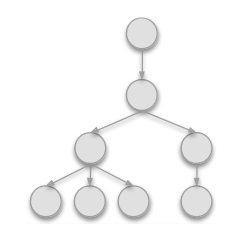
\includegraphics[scale=0.5]{img/albero.png}\\
\g{Tutti i rami} devono essere esaminati fino a quando non viene trovato uno \g{stato di accettazione}.
Come esaminare l'albero:
\textit{in ampiezza} o \textit{in profondità}?

\begin{theorem}
   Per ogni TM \g{non deterministica} esiste una TM \g{deterministica} equivalente
\end{theorem}
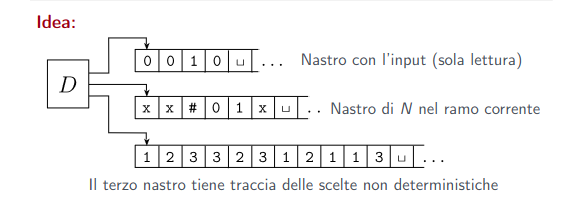
\includegraphics[scale=0.8]{img/idea_non_deterministica.png}

\subsection{Come funziona il terzo nastro }
Ad ogni nodo viene assegnato un \g{indirizzo}: una stringa sull'alfabeto $\Gamma_b = \{1,2,\dots,b\}$, 
dove $b$ è il massimo numero di figli dei nodi dell'albero: \\
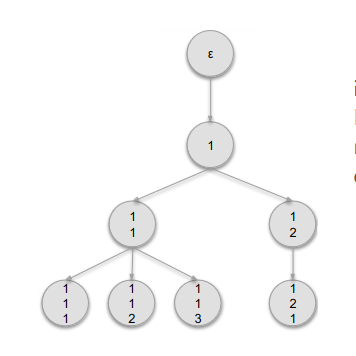
\includegraphics[scale=0.5]{img/albero_2.png}\\
Il nodo 113 si raggiunge prendendo il \g{primo} figlio della radice, seguito dal \g{primo} figlio di quel modo ed infine dal \g{terzo} figlio. 
Questo ordinamento può essere utilizzato per attraversare in modo efficiente l'albero in ampiezza.\\
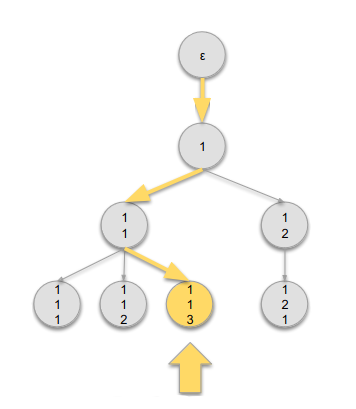
\includegraphics[scale=0.5]{img/albero_3.png}

\subsection{Come funziona $D$}
\begin{enumerate}
   \item Inizialmente il nastro 1 contiene l'input $w$ e i nastri 2 e 3 sono vuoti. 
   \item Copia il nastro 1 sul nastro 2 e inizializza la stringa sul nastro 3 a $\varepsilon$ 
   \item Usa il nastro 2 per simulare $N$ con input $w$ su un ramo di computazione.
      Prima di ogni passo di $N$, consulta il simbolo successivo sul nastro 3 per determinare quale scelta fare (tra quelle consentite).
      Se non rimangono più simboli sul nastro 3, o se questa scelta non è valida, interrompi questo ramo e vai alla fase 4. 
      Vai ala fase 4. anche se si incontra una configurazione di rifiuto.
      Se viene trovata una configurazione di accettazione, \g{accetta}.
   \item Sostituire la stringa sul nastro 3 con la stringa successiva nell'ordine delle stringhe. Simula il ramo successivo di $N$ andando alla fase 2. 
\end{enumerate}

\subsection{Conclusione}
\begin{corollary}
   Un linguaggio è Turing-riconoscibile se e solo se esiste una macchina di Turing \g{non deterministica} che lo riconosce.\\
   $\Rightarrow$ Un linguaggio è Turing-riconoscibile se è riconosciuto da una TM deterministica, che è un caso particolare di TM non deterministica. \\
   $\Leftarrow$ Costruzione precedente 
\end{corollary}

\subsection{Enumeratori}
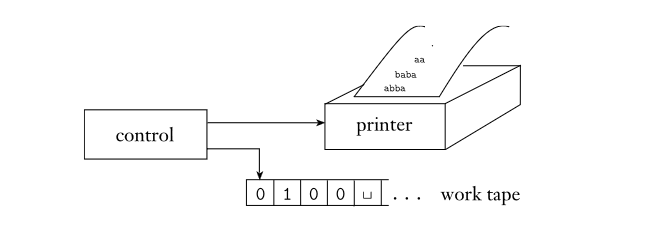
\includegraphics[scale=0.5]{img/enumeratore.png}\\
L'enumeratore è una macchina di Turing che dispone di una stampante.
\begin{itemize}
   \item Un emumeratore $E$ inizia con \g{nastro vuoto}.
   \item Di tanto in tanto, \g{invia una stringa alla stampante} 
   \item Linguaggio \g{enumerato} da $E:$ tutte le stringhe stampate
   \item $E$ può generare le stringhe in qualsiasi ordine, anche con ripetizioni. 
\end{itemize}

\subsection{Equivalenza}
\begin{theorem}
   Un linguaggio è Turing-riconoscibile se e solo se esiste un enumeratore che lo enumera
\end{theorem}
\g{Idea}: dobbiamo mostrare che 
\begin{itemize}
   \item se esiste un enumeratore $E$, allora esiste una TM $M$ che riconosce lo stesso linguaggio 
   \item se esiste una TM $M$ che riconosce il linguaggio, allora possiamo costruire un enumeratore
\end{itemize}

\subsection{Macchine di Turing monodirezionali}
\begin{itemize}
   \item Una macchina di Turing con ``resta ferma'' invece di ``muovi a sinistra''
   \item Funzione di transizione: $\delta : Q\times\Gamma\rightarrow Q\times\Gamma\{S,R\}$ 
   \item Ad ogni passo, la TM può lasciare ferma la testina o muoverla a destra
   \item \textit{Non può muoversi a sinistra}
\end{itemize}

\g{Quale classe di linguaggi riconosce?}

\subsection{Equivalenza con altri modelli}
\begin{itemize}
   \item Esistono altri modelli di computazione universali
   \item Alcuni sono molto simili alle macchine di Turing
   \item Altri sono molto diversi 
   \item Hanno tutti una caratteristica comune:
      \g{accesso senza restrizioni} ad una \g{memoria illimitata} 
   \item Sono \g{tutti equivalenti tra loro} 
\end{itemize}
